\documentclass[11pt]{article}

% font things
\usepackage{amsmath}
\usepackage{MnSymbol} % math things
% serif: if MinionPro doesn't work, use mathptmx
\usepackage[lf, mathtabular, minionint]{MinionPro} % Minion
% \usepackage{mathptmx}   % times
% sans font: use roboto if MyriadPro doesn't work
% \usepackage{MyriadPro} 
\usepackage{roboto}     % sans 


% begin old preamble

% --- character encoding ---
% \usepackage[latin1]{inputenc}
% \usepackage[T1]{fontenc}


\usepackage[top=.8in, bottom=.8in, left=1in, right=1in]{geometry}

% --- old font ---
% \renewcommand{\rmdefault}{pplx}
% \usepackage[sc]{mathpazo}
% \usepackage[OT1, euler-hat-accent]{eulervm}
\usepackage[usenames, dvipsnames, svgnames]{xcolor}
\usepackage{enumitem}

% --- styling ---
\usepackage{titling}
\usepackage[small, compact]{titlesec}
\setitemize[0]{leftmargin=*}
\usepackage{multicol, multirow}
\usepackage{epsfig, subfigure, subfloat, graphicx}
\usepackage{anysize, indentfirst, setspace}
\usepackage{verbatim, rotating, xfrac}
\usepackage{gensymb}
\usepackage{caption, hanging}
\newcommand{\mc}[1]{\multicolumn{1}{c}{#1}}
%\parindent 0pt
%\setdefaultenum{a.}{i.}{A}{1}
%\setdefaultitem{}{\textperiodcentered}{}{}
\usepackage{booktabs}
\usepackage{dcolumn}
\usepackage{caption, hanging}
\usepackage{tikz}
\usetikzlibrary{shapes,arrows,backgrounds}
%\setdefaultenum{a.}{1)}{i.}{a.}
\parindent 0pt

\makeatletter
\newcommand{\distas}[1]{\mathbin{\overset{#1}{\kern\z@\sim}}}%
\newsavebox{\mybox}\newsavebox{\mysim}
\newcommand{\distras}[1]{%
  \savebox{\mybox}{\hbox{\kern3pt$\scriptstyle#1$\kern3pt}}%
  \savebox{\mysim}{\hbox{$\sim$}}%
  \mathbin{\overset{#1}{\kern\z@\resizebox{\wd\mybox}{\ht\mysim}{$\sim$}}}%
}
\makeatother




\title{\Large{\bf{\vspace{-100pt}Mathematics for Political Science \vspace{-15pt}}}}
\author{\large{Lesson 1: Introduction, Foundations, Pre-Calculus}}
\date{\vspace{-5pt}\large{Exercises \vspace{-10pt}}}
\begin{document}
\maketitle

\hrule

\vspace{.5cm}

\begin{enumerate}


\item For the coffeeshop data from lecture, classify each variable variable as:
\begin{enumerate}
\item qualitative or quantitative
\item categorical, ordinal, interval, or ratio
\end{enumerate}


\item Using the data in the table below:
\begin{enumerate}
  \item Find output for the functions $f(x)$ and $g(x)$.
  \item Show the functions equivalent to $f(g(x))$ and $g(f(x))$.
  %f(g(x)) = (7-2x^3)^2 = 49-28x^3 + 4x^6, g(f(x))=2(3-x)^6-4
  \item Find the output for these functions.
\end{enumerate}

\begin{small}
\begin{center}
\begin{tabular}{c|c|c|c|c}
x & $f(x) = (3-x)^2$  & $g(x) = 2x^3 - 4$   & $f(g(x))$  & $g(f(x))$\\ \hline
2 &                   &                     &            &           \\
4 &                   &                     &            &           \\
5 &                   &                     &            &           \\
1 &                   &                     &            &           \\
0 &                   &                     &            &           \\
1 &                   &                     &            &           \\
\end{tabular}
\end{center}
\end{small}


\item Express each of the following complex functions as two simpler functions, one nested inside the other:
\begin{enumerate}
  \item $4(8x-2)^3$ %g(x) = 8x-2, f(x) = 4x^3
  \item $\frac{1}{3x-2}$ %g(x)=3x-2, f(x) = 1/x
\end{enumerate}


\item Explain why there is no ``largest number'' on the interval $(0,1)$.


\item Plot (roughly) the following functions in coordinate space (use separate graphs):
\begin{enumerate}
\item $f(x) = 2x^2$ for $x \in [0,10]$
\item $f(x) = e^{x}$ for $x \in [0,4]$
\item $f(x) = \frac{1}{x}$ for $x \in (0,\infty)$
\item $f(x) = x^3 - x^2 + 1$ for $x \in [0,1]$
\item $f(x)=\left\{\begin{array}{cl}
 -(x^2)  & \textrm{~for~} x \in [-2,0)\\
 \frac{1}{2} & \textrm{~for~} x = 0\\
    x^3 + 1 & \textrm{~for~} x \in (0,2]\\
    \end{array}\right.$
\end{enumerate}



\item (Gill 1.14 [adapted]) The following data are U.S. Census Bureau estimates of population over a 5 year period.

\begin{center}
\begin{tabular}{lr}
Date         & Total U.S. Population \\ \hline
July 1, 2004 & 293,655,404 \\
July 1, 2003 & 290,788,976 \\
July 1, 2002 & 287,941,220 \\
July 1, 2001 & 285,102,075 \\
July 1, 2000 & 282,192,162 \\ \hline
\end{tabular}
\end{center}

Characterize the growth in terms of an approximate parametric expression.  Graphing may help (optional).
% p \approx 282,200,000 + 2,800,000*y


\item Explain in words the difference between a concave and convex function.  Draw one of each to illustrate. 
% conCAVE looks like a cave entrance, conVex looks like a V


\item Characterize the functions below as monotonic or non-monotonic.

\begin{center}
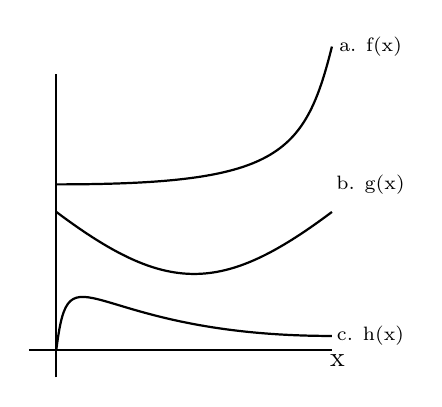
\begin{tikzpicture}[scale=.7]
\draw[thick] (-.5,0) -- (5,0);
\draw[thick] (0,-.5) -- (0,5);
\draw (5.1,-0.2) node{x};
\draw[thick] (0,0) .. controls (.25,2) and (.5,.25) .. (5,.25);
\draw (5.7,.25) node{\scriptsize{c. h(x)}};
\draw[thick] (0,2.5) .. controls (2,1) and (3,1) .. (5,2.5);
\draw (5.7,3) node{\scriptsize{b. g(x)}};
\draw[thick] (0,3) .. controls (4,3) and (4.5,3.5) .. (5,5.5);
\draw (5.7,5.5) node{\scriptsize{a. f(x)}};
\end{tikzpicture}
\end{center}
% a monotonic, b and c not


\item Given the data below, find:
\begin{enumerate}
\item $\displaystyle\sum_1^{10} \frac{m_i}{2}$ %39/2
\item $\displaystyle\prod_1^{6} (m_i - 5$) %-6
\end{enumerate}
\begin{center}
\begin{tabular}{c|c|c|c|c|c|c|c|c|c}
$m_1$  & $m_2$ & $m_3$ & $m_4$ & $m_5$ & $m_6$ & $m_7$ & $m_8$ & $m_9$ & $m_{10}$   \\ \hline
3      & 1     & 8     & 3     & 2     & 7     & 4     & 5     & 4     & 2       \end{tabular}
\end{center}



\item (Gill 1.1 [adapted]) Simplify the following expressions as much as possible (if any simplification is possible):
\begin{center}
\begin{tabular}{p{3cm}p{3cm}p{3cm}}
a. $(-x^4y^2)^2$       &  b. $9(3^0)$                                 & c. $(2a^2)(4a^4)$                     \rule{0cm}{1cm}\\
d. $\displaystyle\frac{x^4}{x^3}$   &  e. $y^3 + y^4 + y^5$                        & f. $\displaystyle\frac{\frac{2a}{7b}}{\frac{11b}{5a}}$ \rule{0cm}{1cm}\\
g. $\ln (\frac{e^4}{3})$& h. $\displaystyle\log_8 1$
\rule{0cm}{1cm}\\
\end{tabular}
\end{center}


\item (Gill 1.2 [adapted]) Simplify the following expressions by expanding the polynomials and grouping like terms:
\begin{enumerate}
  \item $(a+b)^2 + (a-b)^2 + 2(a+b)(a-b) - 3a^2$ %a^2
  \item $3p(q+p)^2 - pq + 4x(q + 2p)^2$ %3pq^2 + 6p^2 q + 3p^3 - pq + x(4q^2 + 16pq +16p^2)
\end{enumerate}


\item Suppose the vote totals a candidate will receive are given by the equation:
\begin{equation*}
V = b + 8s^{\frac{1}{2}}
\end{equation*}
Where $V$ is the number of votes, $b$ is the candidate's number of baseline loyal supports, and $s$ is the amount of money they spend on the campaign.
\begin{enumerate}
\item If candidate A has loyalists $b_A = 20,000$ and spends $s_A = \$1,000,000$, and candidate B has loyalists $b_B = 25,000$ and spends $s_B = \$250,000$, which one will win the election? %B wins 29,000 to 28,000
\item Approximately how would the losing candidate have had to spend to pull even?  How much additional spending is that? % total of 1,265,625, or 265,625 more
\end{enumerate}


% \item (Gill 1.12) Suppose we are trying to put together a Congressional committee that has representation from four national regions.  Potential members are drawn from a pool with 7 from the northeast, 6 from the south, 4 from the Midwest, and 6 from the far west.  How many ways can you choose a committee that has 3 members from each region for a total of 12?\\ % 56,000





\end{enumerate}

\vfill
\begin{center}
\small{Thanks to Dave Ohls, Brad Jones, and Sarah Bouchat for past years' materials}
\end{center}
\end{document} 